L'océan est parcouru par des jets étroits et intenses, comme le Gulf-Stream (océan Atlantique Nord), le Kuroshio (océan Pacifique Nord), ou le courant Pacifique Nord \cite{Talley2011}. Ces jets sont associés à de forts gradients horizontaux de densité/température/salinité (fronts) et sont fortement cisaillés horizontalement. Ces fronts jouent un rôle important dans les transport de chaleur et de quantité de mouvement, et constituent des sites privilégiés en terme de frontogenèse et de génération de structures de sub-méso-échelle \cite{McWilliams2016}. Comprendre les mécanismes à l'origine de la formation et du maintien de ces jets zonaux constitue ainsi un enjeu important de l'océanographie physique.

\begin{figure}[h]
	\centering
	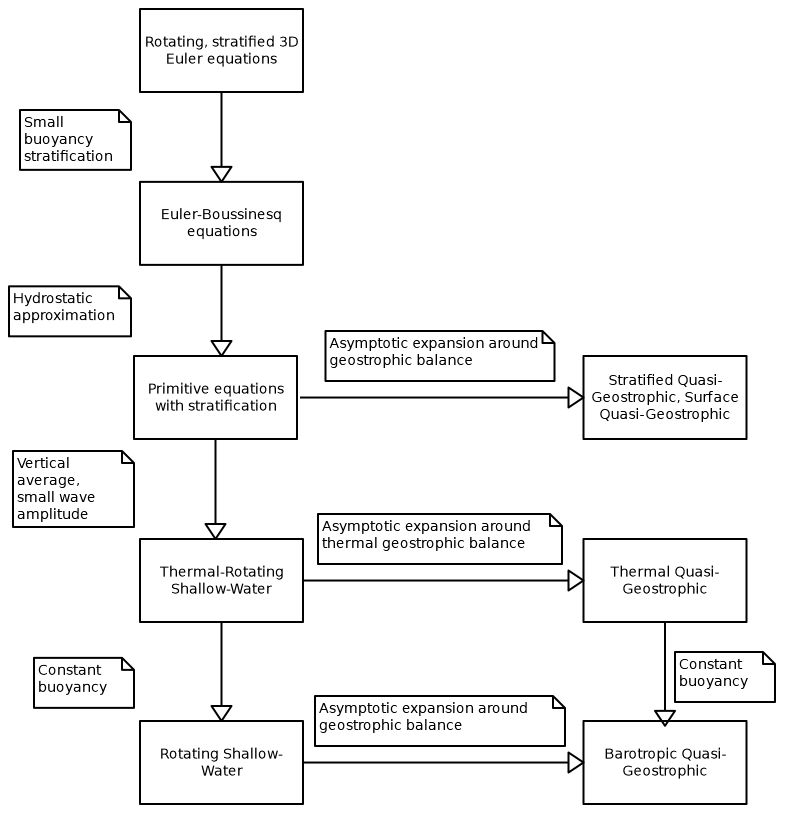
\includegraphics[width=0.5\linewidth]{Figures/diag_eq_holmes.png}
	\caption{Schéma de dérivation de quelque modèles GFD. Adapté de \cite{Crisan2021} et \cite{Holm2021}}
	\label{fig:diag_eq_holmes}
\end{figure}

La complexité de ces phénomènes -qui mêlent dynamique et thermodynamique sur ne large gamme d'échelle- rend leur étude par des modèles océaniques complets coûteuse et peu propice à la détermination des mécanismes physiques sous-jacents. Le recours à des modèles simplifiés constitue donc une approche privilégiée en dynamique des fluides géophysique \cite{CushmanRoisin2011}\cite{Vallis2016}. Ces modèles découlent de simplifications apportées aux équations primitives (figure \ref{fig:diag_eq_holmes}). Le modèle Rotating-Shallow-Water \guillemets{supprime} le problème de la stratification continue, puisqu'il ne considère qu'une ou plusieurs couches de densité constante, tout en permettant la propagation d'ondes rapides (ondes de gravité). Le modèle quasi-géostrophique (QG) \cite{Charney1949}, qui ne s'applique qu'à la dynamique de méso-échelle, va plus loin en filtrant ces ondes rapides : il ne décrit que la dynamique \guillemets{lente} (ondes de Rossby), déterminée par la conservation de la vorticité potentielle. Ce gain de simplicité a quelque limites : le modèle QG stratifié suppose que la flottabilité (et donc la densité) est une variable diagnostique, ce qui limite sa capacité à décrire les fronts. Le modèle Thermal-Quasi-Geostrophic (TQG) \cite{Crisan2021} \cite{Warneford2013} se situe à l'intermédiaire entre le modèle QG strafifié et le modèle QG barotrope. Il couple la conservation de la vorticité potentielle à une équation d'évolution pour la densité (moyennée verticalement), ce qui le rend plus apte à décrire les fronts à méso-échelle.

Malgré leur simplicité relative, ces modèles restent non linéaires et n'ont pas (en général) de solution analytique. A moins de travailler avec des équations linéarisées comme cela se fait pour l'étude du développement des instabilités, le recours à la simulation numérique est donc nécessaire. Leur simplicité présente tout de même l'avantage de nécessiter des ressources de calcul plus réduites que pour des modèles régionaux (ou de circulation générale), ce qui permets de les faire \guillemets{tourner} sur un simple PC de bureau.

Dans ce contexte, le but de ce stage est d'implémenter un modèle TQG afin d'étudier la dynamique des jets zonaux. La première partie présente un \guillemets{panorama} des modèles de type QG, et nous dérivons le modèle TQG. La seconde partie expose en détails la manière dont nous avons résolu numériquement ce modèle. Enfin, la dernière partie présente quelque simulations effectuées avec notre code.
